\documentclass[tikz,border=2pt]{standalone}
\usepackage{amsmath,amssymb}
\usepackage{tikz}
\usetikzlibrary{arrows.meta}

\begin{document}
% Graphical integer programming: draw the continuous constraints, keep only the lattice
% points inside, and pick the one with the best objective by sliding the objective line.
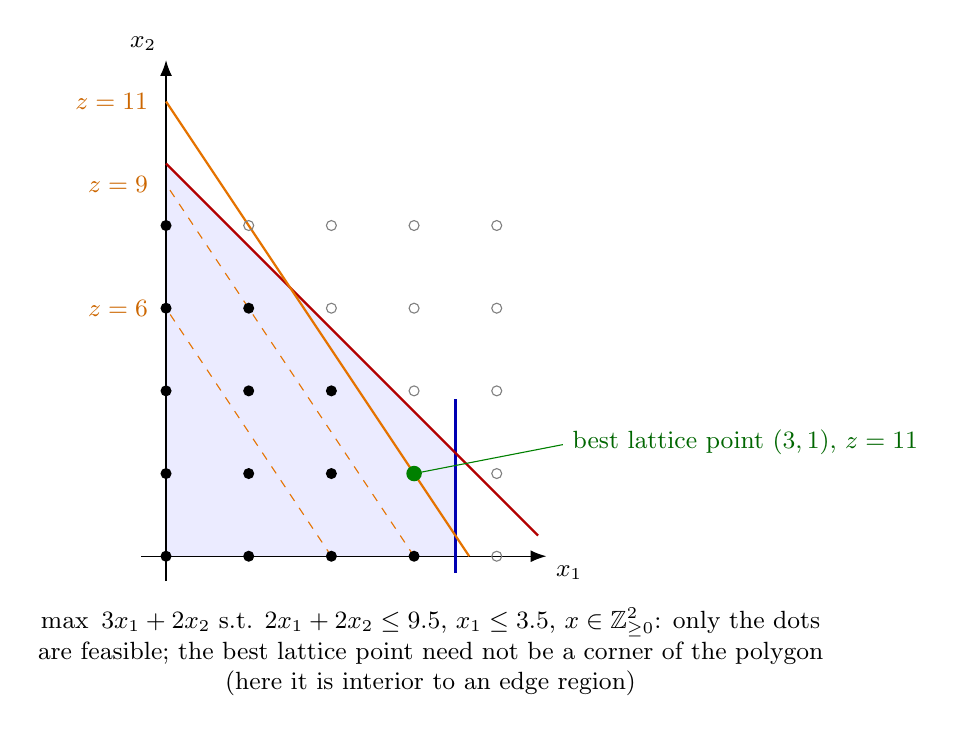
\begin{tikzpicture}[x=1.05cm, y=1.05cm, every node/.style={font=\small}, >={Latex[length=2mm]}]
	\fill[blue!8] (0,0) -- (3.5,0) -- (3.5,1.25) -- (0,4.75) -- cycle;
	\draw[->] (-0.3,0) -- (4.6,0) node[below right] {$x_1$};
	\draw[->] (0,-0.3) -- (0,6.0) node[above left] {$x_2$};
	\draw[blue!70!black, thick] (3.5,-0.2) -- (3.5,1.9);
	\draw[red!70!black, thick] (4.5,0.25) -- (0,4.75);
	\draw[orange!90!black, dashed] (2,0) -- (0,3);
	\draw[orange!90!black, dashed] (3,0) -- (0,4.5);
	\draw[orange!90!black, thick] (3.667,0) -- (0,5.5);
	\node[orange!80!black, font=\small, anchor=east] at (-0.1,3.0) {$z=6$};
	\node[orange!80!black, font=\small, anchor=east] at (-0.1,4.5) {$z=9$};
	\node[orange!80!black, font=\small, anchor=east] at (-0.1,5.5) {$z=11$};
	\foreach \i in {0,1,2,3,4} {\foreach \j in {0,1,2,3,4} {
		\pgfmathparse{(2*\i+2*\j<=9.5 && \i<=3.5) ? 1 : 0}
		\ifnum\pgfmathresult=1 \fill[black] (\i,\j) circle (2pt); \else \draw[gray] (\i,\j) circle (1.8pt); \fi
	}}
	\draw[green!50!black, thin] (3,1) -- (4.8,1.35);
	\fill[green!50!black] (3,1) circle (2.8pt);
	\node[green!40!black, font=\small, anchor=west] at (4.8,1.38) {best lattice point $(3,1)$, $z=11$};
	\node[anchor=north, align=flush center, text width=10cm] at (3.2,-0.5) {$\max\ 3x_1+2x_2$ s.t. $2x_1+2x_2\le9.5$, $x_1\le3.5$, $x\in\mathbb{Z}_{\ge0}^2$: only the dots are feasible; the best lattice point need not be a corner of the polygon (here it is interior to an edge region)};
\end{tikzpicture}
\end{document}
